\section{\color{red}Tekstalgoritmer}
	Generelt problem: Vi er interesserte i å finne ut om en streng er en substreng av en annen streng. Vi kaller substringen for en nål $i$, av lengde $m$, og stringen for en høystakk $h$, av lengde $n$.

	\subsection{Brute force}
		Brute force-metoden er som navnet tilsier ikke spesielt gjennomtenkt: Til å begynne med sjekker vi hver karakter i høystakken mot den første i nåla. Hvis vi har likhet sjekker vi det neste tegnet i høystakken mot det neste i nåla. Vi fortsetter slik til vi enten finner hele nåla i høystakken eller til vi har ulikhet, og i så fall fortsetter vi med å sjekke det neste tegnet i høystakken mot det første i nåla.

	\subsubsection{Analyse}
		Worst case så får vi mismatch $(n-m)$ ganger og suksess $(n-m)+1$ ganger, Totale sammenligninger er $((n-m)+1\times m)$ som gir kjøretid $O(n^2)$.

	\subsection{\color{red}Boyer-Moore}
		Dette er en rask substringalgoritme. Med Boyer-Moore preprosserer vi nåla før vi begynner å søke. Vi regner ut hvor mange hopp vi kan gjøre for hvert enkelt tegn vi får mismatch på. Dette kaller vi \textit{bad character shift}. Vi beregner også \textit{good character shift}, som er verdier vi kan hoppe på et gitt sted i nåla hvis vi har hatt match tidligere i nåla, men ikke på denne plassen. \newline Algoritmen er slik:
		\begin{itemize}
			\item[-] Beregn bad character shift for alle tegn.
			\item[-] Sammenlign nåla med teksten, starter med tegnet lengst til høyre i nåla.
			\item[-] Hvis mismatch på \verb|c|, flytt nåla fram med den \textbf{største} verdien av \verb|badCharShift[c]| og \verb|goodSuffixShift[c]|. Hvis match, dytt nåla en til høyre og sjekk neste tegn. Gjenta.
		\end{itemize}
		Merk at når vi snakker om å skippe så er det alltid i forhold til det siste tegnet i nåla.

	\subsubsection{Bad character shift}
		Vi beregner avstand til neste gang nål er på linje med høystakk\ref{huffman}.
		Ved en mismatch vil vi dytte nåla framover til en av to ting skjer: Mismatch blir match eller nåla beveger seg forbi tegnet vi fikk mismatch på.
		I praksis gjør vi dette slik: Verdien til et tegns bad character shift er lengden på nåla minus den siste indeksen som tegnet befinner seg på, minus 1. Altså \verb|value = length - index - 1|.
		
		\subsubsection*{Eksempel}
		La nåla være ``tooth'', og teksten være ``trusthardtoothbrushes''.
		
		\begin{center}
			\begin{tabular}{c c c c c c}
				& T & O & O & T & H \\
				index & 0 & 1 & 2 & 3 & 4
			\end{tabular}
		\end{center}

		Vi konstruerer bad character shift for denne med regelen \verb|value = length - index - 1|.

\begin{center}
\begin{tabular}{cccl}
T = & $5-0-1$&= 4\\
O = & $5-1-1$&= 3\\
O = & $5-1-2$&= 2&Erstatter her forrige verdi av O med ny verdi til O.\\
T = &$5-3-1$& = 1&Erstatter her forrige verdi av T med ny verdi til T.\\
H = &5 &&Verdien skal ikke være mindre enn 1. Får da verdi lik lengden.\\
\end{tabular}

Vi sitter igjen med dette som bad character shift-tabell: \newline
\begin{tabular}{l|llll}
Bokstav&T&O&H&$*$\\
\hline
Verdi&1&2&5&5\\
\end{tabular}
\end{center}

Vi bruker nå bad character shift på eksemplet vårt: \newline
\scalebox{0.9}{
\begin{tabular}{cccccccccccccccccccccc}
&T&R&U&S&\textcolor{red}{T}&\textcolor{red}{H}&A&R&D&T&\textcolor{red}{O}&O&\textcolor{red}{T}&H&B&R&U&S&H&E&S\\
\textbf{1.}&T&O&O&T&\textcolor{red}{H}\\
\textbf{2.}&&T&O&\textcolor{red}{O}&\textcolor{dkgreen}{T}&\textcolor{dkgreen}{H}\\
\textbf{3.}&&&&&&&T&O&O&T&\textcolor{red}{H}\\
\textbf{4.}&&&&&&&&&T&O&O&T&\textcolor{red}{H}\\
\textbf{5.}&&&&&&&&&&\textcolor{dkgreen}{T}&\textcolor{dkgreen}{O}&\textcolor{dkgreen}{O}&\textcolor{dkgreen}{T}&\textcolor{dkgreen}{H}\\
\end{tabular}
}

I steg \textbf{1.} får vi mismatch på H, fordi den ikke er det samme som T. Da må vi slå opp i tabellen på den bokstaven som \textbf{\textit{vi møter i teksten}}, og hoppe fram tilsvarende antall steg. I første tilfellet skal vi hoppe 1 plass fram (for 1 er verdien til T). 

Sjekker på nytt i steg \textbf{2.}, her får vi match på T og H, men mismatch på O. Da hopper vi S-plasser frem. Siden S ikke er med i tabellen vår (eller den er med som $*$, som er alle andre bokstaver), så hopper vi 5 plasser frem.

I steg \textbf{3.} får vi mismatch på H mot O, og må hoppe O-plasser frem---altså 2. I steg \textbf{4.} er det mismatch mellom H og T, vi hopper T-plasser frem---altså 1. Og nå har vi funnet nåla vår!

\paragraph{Analyse}
Worst case er det samme som brute force. Input tekst $1^n$ kjører $n$ ganger, og nål $011\dots1$ kjører $m$ ganger. Dette gir O($nm$). Best case har input tekst $1^n$ og nål $0^m$, som gir O($n/m$). Average case er O($m/|\Sigma|$), altså raskere enn brute force.
	
	\subsubsection{\color{red}Good suffix shift}
		Anta at vi har en substring $t$ av nåla (altså lengst til høyre i nåla) som allerede er matchet. Vi får så mismatch på neste tegn. Vi kan nå være smarte og finne ut
		Vi må tenke på to tilfeller: $t$ forekommer et annet sted i nåla. Da kan vi ikke skippe lenger enn til neste gang det skjer. Eller, en del av $t$ forekommer i starten av nåla. Da må vi skippe til vi er på linje med dette.
	
		\subsubsection*{Eksempel}
		Vi ser på nåla ``TTCTATTCTT''.

\begin{minipage}{0.5\textwidth}
\paragraph{1.} Sjekker først \textit{ikke}-\texttt{T}, det er to shift før vi finner dette.
\\
\noindent\texttt{TCCTATTCT\textcolor{red}{T}}\\
\texttt{--TCCTATT\textcolor{red}{C}TT}
\\
\paragraph{2.} Så sjekker vi \textit{ikke}-\texttt{TT}. Dette finner vi etter ett shift.
\\
\noindent\texttt{TCCTATTC\textcolor{red}{TT}}\\
\texttt{-TCCTATT\textcolor{red}{CT}T}
\\
\paragraph{3.} For å finne \textit{ikke}-\texttt{CTT} må vi flytte 3 steg; til \texttt{ATT}.
\\
\noindent\texttt{TCCTATT\textcolor{red}{CTT}}\\
\texttt{---TCCT\textcolor{red}{ATT}CTT}
\end{minipage}
\hspace{10pt}
\begin{minipage}{0.5\textwidth}
\paragraph{4.} Så kommer vi til \textit{ikke}-\texttt{TCTT}. Denne eksisterer ikke, MEN om nålen har lik suffix som prefiks (her \texttt{T} som start og slutt), så flytter vi bare fram til prefiksen. Da må vi flytte nålen 9 hakk, selv om lengden er 10.
\\
\noindent\texttt{TCCTATTCT\textcolor{red}{T}}\\
\texttt{---------\textcolor{red}{T}CCTATTCTT}
\\
Alle de neste shiftene vil også være dette, fordi de får ingen andre treff i nålen.
\end{minipage}

\vspace{10pt}

\noindent Vi får da følgende good suffix table:
\begin{table}[H]
\centering
\begin{tabular}{crc}
index&mismatch&shift\\
\hline
0&\texttt{\textcolor{red}{T}}&2\\
1&\texttt{\textcolor{red}{T}T}&1\\
2&\texttt{\textcolor{red}{C}TT}&3\\
3&\texttt{\textcolor{red}{T}CTT}&9\\
4&\texttt{\textcolor{red}{T}TCTT}&9\\
5&\texttt{\textcolor{red}{A}TTCTT}&9\\
6&\texttt{\textcolor{red}{T}ATTCTT}&9\\
7&\texttt{\textcolor{red}{C}TATTCTT}&9\\
8&\texttt{\textcolor{red}{C}CTATTCTT}&9\\
9&\texttt{\textcolor{red}{T}CCTATTCTT}&9\\
\end{tabular}
\caption{Eksempel på good suffix table.}
\label{tab:gst}
\end{table}

	\subsection{Huffmankoding}\label{huffman}
		Huffmankoding er en måte å kode informasjon på (her tekst) på en måte der vi ikke mister noe informasjon (\textit{lossless}). Den forutsetter at vi har tilgang på teksten før vi lager en kode. Dette er ikke tilfellet med vanlig tekstenkoding, der hvert tegn har en standard kode. Huffmankoding går ut på å se på frekvensen til tegnene som forekommer, og gi kort kode til de tegnene som forekommer ofte, og lang kode til de som forekommer sjelden. Dette kan vi gjøre slik at vi har prefiksegenskapen intakt: Ingen koder er et prefiks av noen andre. Kodealfabetet \{9, 55\} har prefiksegenskapen, men \{9, 5, 59, 55\} har ikke. Måten Huffmankoding beholder denne egenskapen blir fort tydelig når vi ser på algoritmen. Kort fortalt er grunnen at vi benytter binære trær til å finne kodene.
		
		Algoritmen:
		\begin{enumerate}
			\item Lag frekvenstabell for alle tegn som forekommer i teksten.
			\item Betrakt hvert tegn som en node som skal settes sammen til et tre, og legg alle noder i en prioritetskø (heap. Se \ref{heap}) $P$.
			\item Mens $P$ har mer enn ett element:
				\begin{itemize}
					\item[-] Ta ut de to minste nodene fra $P$.	
					\item[-] Gi disse to en foreldernode med vekt lik summen av de to nodene.	
					\item[-] Legg foreldrenoden inn i $P$.	
				\end{itemize}
				Når dette er ferdig har vi et binært tre. Merk at det finnes svært sjeldent et entydig tre!
			\item Vi leser koden til et tegn ved å følge stien fra rotnoden ned til tegnets løvnode. Vi får en `0' når vi går til venstre, og en `1' når vi går til høyre. (Dette fungerer selvfølgelig ved å gjøre motsatt, så lenge man er konsekvent.) Merk igjen at det svært sjelden finnes entydige koder, men med denne algoritmen vil de uansett være optimale.
		\end{enumerate}
		Algoritmen burde bli klar når vi ser på et eksempel.

		\begin{eks}
		Anta at vi har en tekst ``BACADAEAFABBAAAGAH''. Vi setter opp en frekvenstabell for bokstavene i koden.
			\begin{center}
				\begin{tabular}{c c c}
					Tegn & Frekvens \\
					\hline
					A & 9\\
					B & 3\\
					C & 1\\
					D & 1\\
					E & 1\\
					F & 1\\
					G & 1\\
					H & 1
				\end{tabular}
			\end{center}
			Vi ser at vi kan parvis slå sammen to og to av nodene som har vekt 1: Vi slår sammen C og D, E og F, og G og H. Nå har (CD), (EF) og (GH) alle vekt 2. Vi slår så sammen B og (CD) til en node (B, CD) med vekt 5, og vi slår sammen (EF) og (GH) til en node (EF, GH) med vekt 4. Vi slår så igjen sammen (B, CD) og (EF, GH) slik at de får en foreldrenode med vekt 9. Til slutt slår vi sammen denne med noden A. Det resulterende treet er:

			\begin{figure}[H]
				\centering
				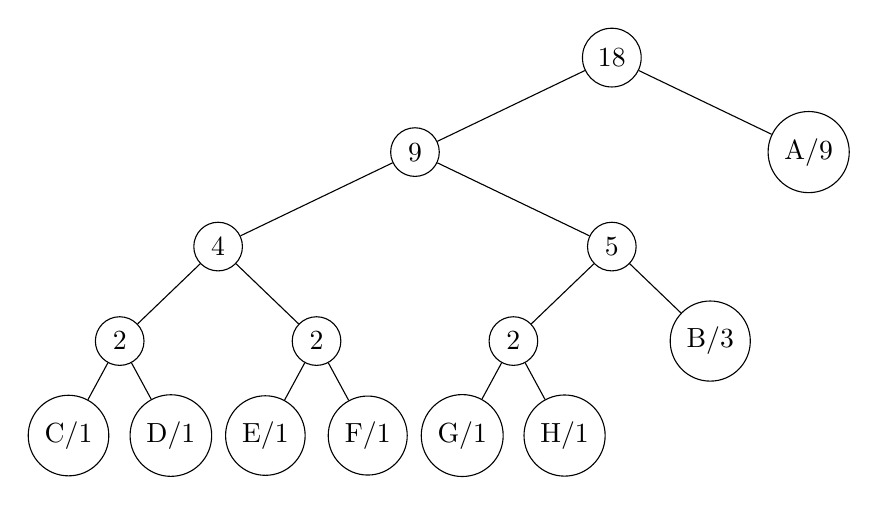
\begin{tikzpicture}[level distance=1.2cm,
				level 1/.style={sibling distance=5cm},
				level 2/.style={sibling distance=5cm},
				level 3/.style={sibling distance=4cm},
				level 3/.style={sibling distance=2.5cm},
				level 4/.style={sibling distance=1.3cm}
				]
				\tikzstyle{every node}=[circle,draw]
				
				\node {18}
					child {
					node {9} 
					child {
				    	node {4}
				    	child { node {2}
				    	child {node {C/1}}
				    	child {node {D/1}}}
				    	child { node {2}
				    	child {node {E/1}}
				    	child {node {F/1}}}
					}
					child {
				    	node {5}
				    	child { node {2}
				    	child {node {G/1}}
				    	child {node {H/1}}}
				    	child { node {B/3}
				    	}
					}
						}
					child {
					node {A/9}
					}
				;
				\end{tikzpicture}
			\end{figure}

			Hvis vi nå følger regelen fra algoritmen om å skrive `0' når vi går venstre og 1 når vi går høyre får vi kodene:
			\begin{center}
				\begin{tabular}{c c c}
					Tegn & Frekvens & Kode \\
					\hline
					A & 9 & 1\\
					B & 3 & 011\\
					C & 1 & 0000\\
					D & 1 & 0001\\
					E & 1 & 0010\\
					F & 1 & 0011\\
					G & 1 & 0100\\
					H & 1 & 0101
				\end{tabular}
			\end{center}
			Vi kan lett sjekke at prefiksegenskapen er intakt, og teksten ``BACADAEAFABBAAAGAH'' får koden \verb|011100001000110010100111011011111010010101|. Dette er åpenbart mye kortere enn standard enkoding. Hvis vi for eksempel hadde brukt ASCII-enkoding, der hvert tegn har en 7-bits kode, hadde vi hatt en kode på lengde $7n$, der $n$ er lengden på teksten.
			\end{eks}